\documentclass[12pt,oneside]{fithesis2}
\usepackage{graphicx}
\usepackage[english]{babel}       % Multilingual support
\usepackage[utf8]{inputenc}       % UTF-8 encoding
\usepackage[T1]{fontenc}          % T1 font encoding
\usepackage[                      % A sans serif font that blends well with Palatino
  scaled=0.86
]{berasans}
\usepackage[                      % A tt font if you do not like LM's tt
  scaled=1.03
]{inconsolata}
\usepackage{blindtext}
\usepackage[hyphens]{url}
\usepackage[                      % Clickable links
  plainpages = false,               % We have multiple page numberings
  pdfpagelabels,
  hidelinks                     % Generate pdf page labels
]{hyperref}            % Lorem ipsum generator
\usepackage{listings}
\usepackage[svgnames]{xcolor}

\usepackage{amsthm}
\newtheorem{definition}{Definition}

\usepackage{ftnxtra}
\usepackage{fnpos}

\definecolor{javared}{rgb}{0.6,0,0} % for strings
\definecolor{javagreen}{rgb}{0.25,0.5,0.35} % comments
\definecolor{javapurple}{rgb}{0.5,0,0.35} % keywords
\definecolor{javadocblue}{rgb}{0.25,0.35,0.75} % javadoc
\definecolor{maroon}{rgb}{0.5,0,0}
\definecolor{darkgreen}{rgb}{0,0.5,0}

\lstdefinestyle{eclipse_java}
{
	language=Java,
	basicstyle=\ttfamily,
	keywordstyle=\color{javapurple}\bfseries,
	stringstyle=\color{javared},
	commentstyle=\color{javagreen},
	morecomment=[s][\color{javadocblue}]{/**}{*/},
	tabsize=4,
	showspaces=false,
	showstringspaces=false
}


\lstdefinestyle{my_xml}
{
	language=XML,
	basicstyle=\ttfamily,
	morestring=[s]{"}{"},
	morecomment=[s]{?}{?},
	morecomment=[s]{!--}{--},
	commentstyle=\color{darkgreen},
	moredelim=[s][\color{black}]{>}{<},
	moredelim=[s][\color{red}]{\ }{=},
	stringstyle=\color{blue},
	identifierstyle=\color{maroon},
	tabsize=2,
	showstringspaces=false
}

\lstdefinestyle{json}
{
	basicstyle=\ttfamily,
	tabsize=2,
	showstringspaces=false,
	keywordstyle=\bfseries,
	morekeywords={thrown}
}

\lstdefinestyle{byteman}
{
	tabsize=2,
	showstringspaces=false,
	basicstyle=\ttfamily,
}

\lstset{frame=lrtb, captionpos=b, breaklines=true, showstringspaces=false, basicstyle=\ttfamily}
\lstset{language=Java}
\lstset{language=XML}

\usepackage[chapter]{minted}

\usepackage{multicol}
\usepackage{enumitem}
\usepackage{nameref}

\thesislang{en}                   % The language of the thesis
\thesistitle{Monitoring Extension for Microservices Platform SilverWare}       % The title of the thesis
\thesissubtitle{Diploma Thesis}  % The type of the thesis
\thesisstudent{Bc. Jaroslav Dufek}          % Your name
\thesiswoman{false}                % Your gender
\thesisfaculty{fi}                % Your faculty
\thesisyear{\the\year}     % The academic term of your thesis defense
\thesisadvisor{Mgr. Martin Večeřa}   % Your advisor

\begin{document}
  \FrontMatter                    % The front matter
    \ThesisTitlePage                % The title page
    \begin{ThesisDeclaration}       % The declaration
      \DeclarationText
      \AdvisorName
    \end{ThesisDeclaration}
    \begin{ThesisThanks}            % The acknowledgements (optional)
      Doplnit podekovani.
    \end{ThesisThanks}
    \begin{ThesisAbstract}          % The abstract
    
    
    UPRAVIT 

    
The aim of this thesis is to design and implement monitoring extension for microservices platform Silverware. At the beginning I study current most known microservices platforms and research how they implemented their monitoring part. Then I come up with possible monitoring solution for SilverWare that would be appropriate for the scope of this thesis. Lastly I implement this solution using Hawtio platform as a front-end.
    \end{ThesisAbstract}
    \begin{ThesisKeyWords}          % The keywords
      DOPLNIT
    \end{ThesisKeyWords}
    \tableofcontents                % The table of contents
%   \listoftables                   % The list of tables (optional)
%   \listoffigures                  % The list of figures (optional)
  
  \MainMatter                     % The main matter
\chapter{Introduction}

\section{Goals and challenges}

My overall goal was to explore very young realm of services and applications written as microservices with focus on monitoring such systems and consequently implement a monitoring provider extension for one of the microservice frameworks called SilverWare.

Because this field was completely new to me, I first needed to read some introduction books to even get a grasp of what microservices are, why is everyone so excited about them, what are their core principles, what can they offer and what challenges they come with.

Afterwards I learned basics regarding containerization of applications and their usage with focus on OpenShift/Kubernetes/Docker platform which provide fitting environment for microservice applications and are very often mentioned in various articles. Then I briefly tried out contemporary microservice frameworks and platforms and finally got my hands on SilverWare which code and internal workings I needed to study thoroughly so I could develop suitable extension for it.

When I had sufficient general insight into the microservices landscape I steered my attention towards actual monitoring issues of microservices and looked for appropriate standards and solutions which I could integrate into the SilverWare microservice framework.

\section{Structure of the Thesis}

DOPLNIT NA KONCI

\chapter{Microservices}

For many years now, we have been finding better ways to build systems. We have been learning from what has come before, adopting new technologies, and observing how a new wave of technology companies operate in different ways to create IT systems that help make both their customers and their own developers happier. \cite{ma}

Software systems have become more and more complex as their scale increased. Scale in the form of scope, volume, and user interactions. This increase of scale has brought many problems upon traditional way of developing enterprise applications. Problems such as increased complexity of the software and so increased development time, tight coupling of system parts and so inability to change, increased deployment dependencies and deployment time. Microservices try to tackle these problems and many more.

Microservice architecture has emerged as a common pattern of software development from the best practices of a number of leading organizations and their endeavor of building big and continually growing, maintainable and adaptable enterprise systems which are able to swiftly react to ever-changing software requirements.

\begin{definition}[Microservice architecture (MSA)]
A microservice architecture is a distributed application where all its modules are microservices. \cite{mytat}
\end{definition}

\begin{definition}[Microservice]
A microservice  is  a  minimal  independent  process  interacting via messages. \cite{mytat}
\end{definition}

Microservice architecture is an approach to modularization of software. Modularization itself is nothing new. For quite some time large systems have been divided into smaller components to facilitate the implementation, understanding and further development of the software. However microservice architecture utilizes experience gained by developers over the years to take the modularization to a new level.

Microservices-based architecture is a development concept which advocates decomposing business domain models of a system into smaller, consistent, bounded-contexts implemented by a collection of small, isolated services. Each of these services owns their data, and is independently scalable and resilient to failure. These small services or so called microservices integrate with each other in order to form a united system that is far more flexible than the typical monolithic enterprise systems we build today. \cite{rma}

Previous technical limits held us back from implementing the concepts embedded within the microservices: single machines running single core processors, slow networks, expensive disks, expensive memory, and organizations structured as monoliths. But now the technology has matured and enabled us to take the development of big enterprise software to the next level.

So to recapitulate - the basic idea of microservices is instead of building a single monstrous, monolithic application we should split the application into a set of smaller, interconnected services each of which takes care of part of the functionality provided by the system and is easily replaceable.

\section{Breaking the monolith}

One good way to present microservices in more detail is by showing the differences between them and conventional applications regarding development, deployment, operation and so on. In order to do that we should first recollect how the conventional business applications work.

Traditional enterprise systems are designed as monoliths -- all-in-one, all-or-nothing. They are difficult to scale, difficult to understand and difficult to maintain.

\begin{definition}[Monolith]
A monolith is a software application composed of modules that are not independent of the application to which they belong. \cite{mytat} 
\end{definition}

Evergrowing monoliths can quickly turn into nightmares that stifle innovation, progress, and joy. Negative side effects of monoliths can be catastrophic for a company. They can derogate morale of a team, discourage talented people from entering the team, cause high alternation of employees which in turn causes outflow of people that already understood the complex system which further deepens the lack of understanding of monolith. All this can in the worst cases even lead to the failure of a company due to inability to react to change. \cite{rma}

\paragraph{Enterprise applications are often composed of three main parts:}

\begin{enumerate}
   \item a client-side application - which can either be a webpage running in a  browser on the user's machine communicating with the webserver using HTTP  protocol or a smartphone applications communicating using REST protocol
   \item a server-side application - consisting of webserver coupled with all business application logic
   \item a database - consisting of many tables inside a common, usually relational, database which often resides on the same machine
\end{enumerate}

\begin{figure}[ht!]
	\centering
	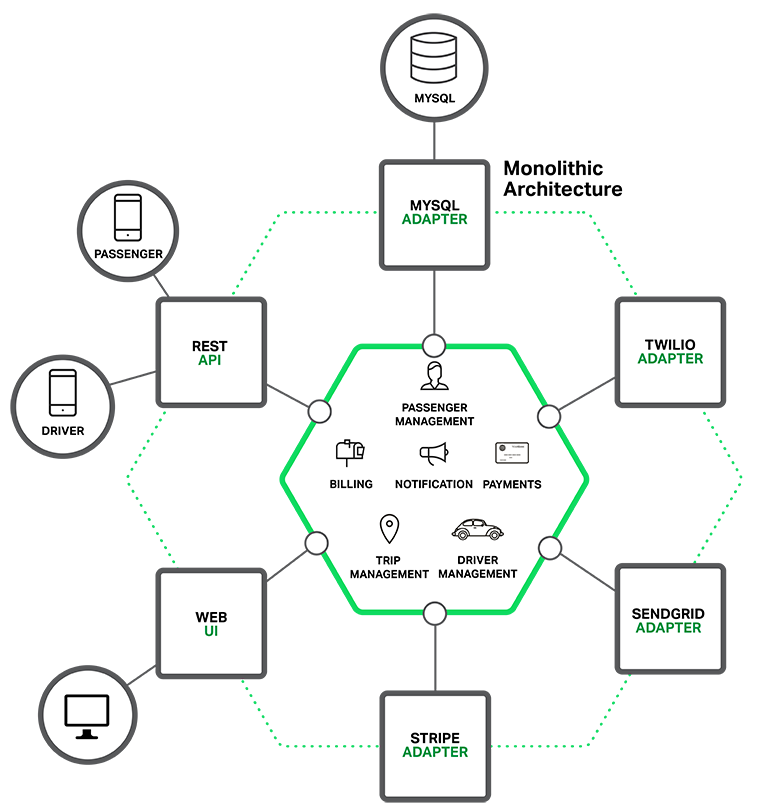
\includegraphics[width=\textwidth]{images/monolithic_application2.png}
	\caption{Monolithic application\footnotemark}
	\label{monolithic_application}
\end{figure}

\footnotetext{Source: \url{https://www.nginx.com/blog/introduction-to-microservices/}}

The server-side application handles all client requests, executes business logic, retrieves and update data from the database, and select and populate HTML views to be sent to the browser. This server-side application is a monolith (as shown in \ref{monolithic_application}) - a single logical executable. Any changes to the system involve building and deploying a new version of the application to the server. \cite{mf}

Monolithic application are typically developed by one, potentially big, team. All requests for change are aggregated into a single issue-tracking system from which the members of team pick their tasks. Likewise the whole team is sharing application`s code-base through a single repository. When members pick their task, they pull current version of the code-base, compile it and start a local development instance on their machine. When they are done with their tasks, they merge their individual changes to the shared repository, thus conflicting changes may be common. In certain time current state of the code-base is marked with a version number and then compiled and deployed to testing environment where it is tested and cultivated for some time before it is finally deployed to production.

Every change in large monolith can be cumbersome. Monoliths allow programmers to strongly couple their code. Change in one part of the application can immediately break something different or have unforseen consequences later. Refactoring of code becomes a pain.

Deployment of monolithic applications can be demanding due to conflicting  requirements on resources. Some of the modules can be processor-intensive, others memory-intensive, storage-intensive or network-intensive. Some modules may require ad-hoc software components like third-party software or different types of databases. Deployment environment then must supply all these needs at once which either leads to expensive or sub-optimal solution.

Monoliths also bring unnecessary overhead when scaling beyond a single machine, this is called horizontal scaling. There are two types of scaling: vertical and horizontal. Vertical scaling means that we are allocating more computing resources within a given machine to the application or you are upgrading the machine itself, this is the ordinary type of scaling. However, vertical scaling is always limited by technical limits of contemporary computer components. Furthermore price of those components rises exponentially together with their performance.

On the other hand with horizontal scaling we are running the same application on multiple machines at once. This solution also necessitate the use of intermediate machine called load-balancer which splits the incoming requests between all the running applications on different machines. The downside of monolith is that even if the bottleneck of your application lies in a single component, you have to run multiple instances of the whole thing claiming more resources. Another problem is even if we utilize horizontal scaling, all the running monoliths share a single database, which then becomes bottleneck by itself.

Now when we look at the microservice architecture we will see a very contrasting mindset. Microservice architecture advocates slicing the monolithic application into well bounded, smaller application parts - microservices that can each provide a part of the business value on their own. This process has been termed as \textit{"breaking the monolith"}. By providing business oriented APIs to user a collection of microservices then substitute the monolith.

As we see in figure \ref{microservice_application}, we broke the application from previous picture into individual components and exposed their APIs through API gateway to client-side applications. Each component can have numerous running copies on different computers (horizontal scaling) and API gateway serves as a load-balancer routing the incoming traffic to them. The only relation between different components is their communication using data exchange accomplished through the APIs they expose. How exactly you slice the business functionality depends on you, but you should try to make the microservices as independent as possible so they limit one another the least.

\begin{figure}[ht!]
	\label{microservice_application}
	\centering
	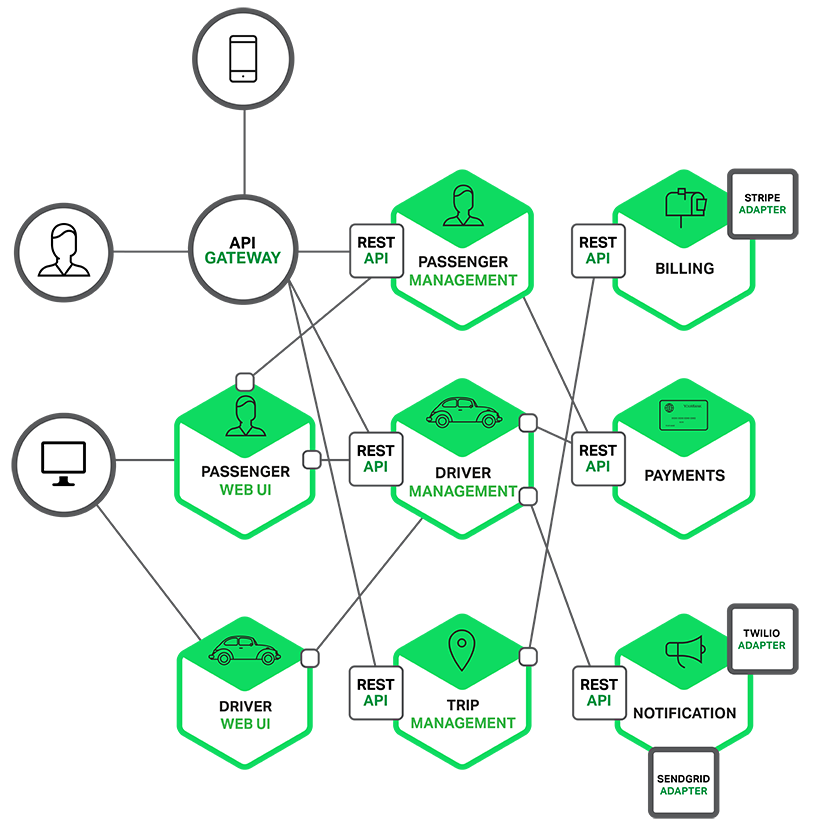
\includegraphics[width=\textwidth]{images/microservice_application2.png}
	\caption{Application as microservices\footnotemark}
\end{figure}

\footnotetext{Source: \url{https://www.nginx.com/blog/introduction-to-microservices/}}

Microservices architecture is not precisely defined in any book, it is not a standard. It is just a set of practices and recommendation that has been put together over time by companies and experts that were facing common problems when building large scale applications. There are key principles that microservice application should stick to.

\subsection{Single responsibility principle}

One of the key principles is that a microservice should do only one thing and it should do it the best it can. This principle is inspired by the philosophy of UNIX where there are many small programs, each of them serves single small purpose and they work together to complete more complicated tasks.

This attitude contributes to microservices staying simple and seizable. They can be maintained by small teams, composed of only a handful of people, that have very good understanding of all aspects of the microservice. Code-base remains small, easy to change and to refactor.

\subsection{Isolation}

Microservices should be as isolated as possible. Isolation means that there are no common resource like a single database between microservices. It also means that every microservice has its own code-base. No relation exist between microservices other than a possibility of communication through arranged interfaces. Low coupling is crucial for many of the microservices benefits.

\subsection{Data ownership}

Part of the isolation principle is data ownership. Every microservice should be responsible for its own data and be able to manipulate it how it deems fit and even change it completely disregarding other microservices. Any other microservice can access these data only through the respective microservice that owns it.

Example of this may be e-shop application where catalog microservice owns only data regarding all offered goods like their id, name, price, description and all kinds of attributes. Then we would have storage microservice that would own data quantity of each item in our stock. Cart microservice which would keep track of users shopping carts. Orders microservice which would take care of customer orders. Login service, images service, recommendations, invoices, etc.
Every microservice would store its data in its own database or hold it in cache. This principle is necessary so that one shared database would not become another bottleneck of the application and single point of failure.

In picture \ref{decentralised_data} we can see difference in data handling between monolithic application and microservice application. On the left side all-inclusive application accesses one big database, performs some business functionality on it and returns the overall result to the user usually in the form of complete web page. On the right side individual microservices serve their respective data either to some front-end web server application or directly to client-side AJAX\footnote{Asynchronous Javascript and XML \url{https://en.wikipedia.org/wiki/Ajax_(programming)}} application or smartphone app. We can also see that there are two instances of the same microservice sharing one database.

\begin{figure}[ht!]
	\label{decentralised_data}
	\centering
	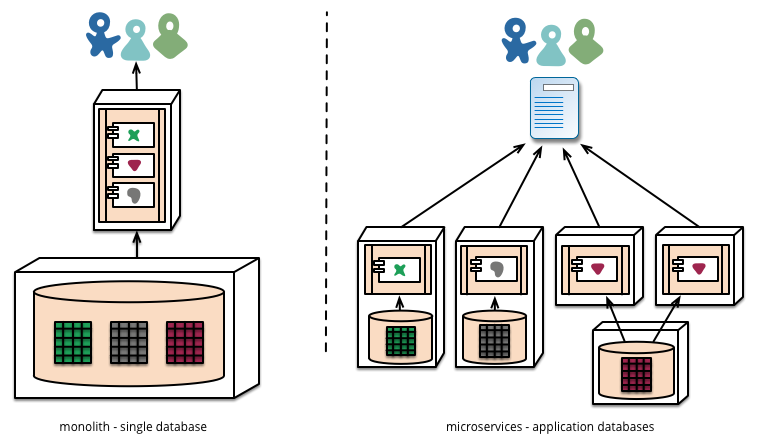
\includegraphics[width=\textwidth]{images/decentralised_data.png}
	\caption{Data division \cite{mf}}
\end{figure}

\subsection{Autonomy}

This principle says that the microservice should be able to exist on its own. Isolation is a prerequisite for autonomy. Only when services are isolated they can be fully autonomous and act independently. No other microservice in the system has to be running for a microservice to run.

Autonomous microservices open up flexibility around orchestration, scalability and availability. Each team and service can change its internal implementation details without impact across the rest of the system. Each service is developed, tested and deployed independently.

\subsection{Resilience}

With previous point ties another characteristic - resilience. Resilience is a capability to cope with unpredictable external changes or errors. A microservice cannot rely on other microservices or components that they will do their job.
In microservice world that encourages autonomy, there are many things that can go wrong. Instances of microservices start and stop on regular basis. It may even happen that in one moment there are no running instances at all - for example when the whole system is just starting. Other microservice can return errors or unexpectedly stop short in the middle of request. Since microservices are typically deployed across multiple machines in a network, all network problems need to be taken into account.

A microservices should also degrade gracefully. Which means that if another component it relies on wasn`t able to provide its promised service, the reliant microservice gradually cuts some of its functionality but tries to leave the most of it, providing the best possible service it can in any given time.

\subsection{Light-weight communication}

Since microservices complete more complicated tasks only by cooperation, there are heavy demands on communication, both in frequency and volume. Thus communication between microservices must be as light-weight as possible. Communication protocols like SOAP that uses bloated XML format are undesirable. Instead microservices architecture recommends usage of protocols like REST that use shorter JSON format.

Some are taking things even further and advocate using a message-oriented approach for communication between microservices. Instead of sending serialized “objects” of agreed format through given entry-points, microservices expose general entry-point for sending task-specific messages allowing for changes in message content. This further helps to reduce coupling and allows safe refactoring.

For example Netflix relies on even smaller message formats like Apache`s Avro or Thrift and Google`s Protobuf over TCP/IP for internal communication inside microservice systems. \cite{ma}

\subsection{Continuous integration}

\begin{definition}[Continuous integration]
Continuous integration is a software development practice where members of team integrate their work multiple times per day and automatic build and test tools check the functionality of the application. \footnote{Continous integration by Martin Fowler \url{https://martinfowler.com/articles/continuousIntegration.html}}
\end{definition}

The goal of continuous integration is reduction of risk, it protects the development from surprises at the end of the development cycle. Waiting days or weeks to integrate code creates many merge conflicts, hard to fix bugs, diverging code strategies, and duplicated efforts. It also provides helpful feedback for both developers and customers.

\paragraph {Key practices that enable continuous integration are:}

\begin{itemize}
\item \textbf{code-versioning} - use of modern code repositories like Subversion or Git is the standard in all good development practices
\item \textbf{frequent commits} - developers should commit their changes and checkout changes of others several times a day to reduce conflicts, it is even recommended not to use branching features for every task and work only on master branch
\item \textbf{automated builds and tests} - each integration (each commit to repository) should trigger an automated self-testing build that verifies the application using unit tests and other means to detect integration errors as soon as possible, it should be easy to see what changes made the build break
\item \textbf{fast builds} - the main point of CI is to provide rapid feedback, so keeping the build times as short as possible is imperative, luckily small scope and size of microservices favours this
\item \textbf{prepare to deliver} - after every successful build or at least every day, new version of application should be pushed to testing environment so there is enough time before deploying to production when testers can spot out errors and stakeholders can adjust imperfections
\item \textbf{testing in clone of production} - having a test environment that is different from production environment can lead to unexpected failures when finally deploying to production, so these two should be as much same as they can be, another solution is to have a pre-production environment
\end{itemize}

\subsection{Utilization of infrastructure}

Microservices architecture encourages pushing common concerns like management and monitoring of the running application to technical infrastructure and framework. Developers should only need to care about business logic.
Automated service discovery and routing should facilitate decoupling of services and enable easy upgrade and replacement.

\subsection{Conway`s Law}

Conway`s law is not a characteristic of microservice architecture but it is a difficulty that needs to be taken into account when designing one.

\begin{definition}[Conway`s law]
Any organization that designs a system (defined broadly) will produce a design whose structure is a copy of the organization’s communication structure. \footnote{How Do Committees Invent \url{http://www.melconway.com/Home/Committees_Paper.html}}
\end{definition}

This finding warns against instinctive pitfall of designing individual microservices and the communication between them based on the preimage of existing teams in the company and their communication.

For example if we had three teams that are specialized respectively on UI, back-end and databases, they would be naturally inclined to develop three microservices - one for serving webpages only acting as a webserver, another executing all business logic and last one for accessing the database. This would be a wrong distribution of responsibilities. Every change in the system would most certainly need modification of all three microservices.

\section{Microservices vs Service Oriented Architecture}

\url{http://stackoverflow.com/questions/25501098/difference-between-microservices-architecture-and-soa}
Microservices Flexible Softwar Architecture ma dobry rozdily

Microservice architecture is heavily inspired by service-oriented architecture (SOA). Some say microservices is a specialization of SOA. Service-oriented architecture is an interlink between monolithic systems and microservices. Both MSA and SOA are architecture patterns that place a heavy emphasis on services as the primary architecture component used to implement and perform functionality. However the crucial difference between them is that microservices architecture is a share-as-little-as-possible architecture pattern that places a heavy emphasis on the concept of a bounded context, whereas SOA is a share-as-much-as-possible architecture pattern that places heavy emphasis on abstraction and business functionality reuse. \cite{mvsoa}

SOA`s focus on reuse means that one certain function should only exist in one place or that single service should handle it. Where things differ is definition of this function. This is where cohesion comes into play. Cohesion is the degree in which functionality in services belongs together. The highest cohesion is functional cohesion where the services contribute to a well-defined task or business capability. Microservices aim for high (functional) cohesion, whereas SOA uses low (logical) cohesion. Logical cohesion means that services are designed to provide similar tasks. This leads to services such as "data service"  which provides all communication with a database for the whole system. Now imagine the effects of this service going down. All parts of the system that persistently store data to database would stop working. With MSA the intention is to provide all aspects of business capability end-to-end, from data storage to user interface functions. So instead of having a "front-end service" and “data service” we have “customer service” and “shipping service” each with their own front-end and back-end part, including database.

MSA also strives for autonomy which not only means that a microservice should be able to run or function independently, but it also means that a microservice should be able to provide business value on its own.

\paragraph{Lets summarize the key differences:}

\begin{itemize}
\item \textbf{Communication between services:} SOA usually has more dependent ESB (Enterprise Service Bus), whereas microservices use faster messaging mechanism, usually REST
\item \textbf{Programming style:} SOA encourages imperative programming, whereas microservices encourages responsive-actor programming
\item \textbf{Database:} SOA models tend to have an outsized relation database, while microservices frequently use NoSQL or micro-SQL databases (which can be connected to conventional databases)
\end{itemize}


\section{Advantages and disadvantages}

Now that we have a general idea of what microservices are, we should look at their benefits and pitfalls, and why is the industry so excited about them.

As Martin Fowler points out \cite{mf}, Netflix, eBay, Amazon, the UK Government Digital Service, realestate.com.au, Forward, Twitter, PayPal, Gilt, Bluemix, Soundcloud, The Guardian, and many other large-scale websites and applications have all evolved from monolithic to microservices architecture. So there must be certainly a good reason for these companies to prefer microservices architecture over monolithic architecture in some of their projects.

\paragraph{The Benefits of Microservices}

\subsection{Long-term maintainability}

Microservices tackle the monoliths specific complexity in its tight coupling between individual, great amount of overall knowledge needed to make responsible changes to the system, technology lock-in, growing technology debt and so on.

When the monstrous monolithic application is broken up into manageable chunks it is easier for everyone in the project to work with the application and further maintain it. Maintainability is absolutely critical for success of big long-lasting projects and represents a great risk if not taken into account.

\subsection{Independent and horizontal scalability}

Evident advantage of microservice architecture is its adaptation to scaling. Isolation and autonomy of a microservice allow us to simultaneously run countless copies of it in addition to running them across different computers in a network.

So for example, if our application has to process computational-intensive task and this task is a responsibility of one of our microservices, we can run that given microservice as many times as we need to satisfy the demand for given task without scaling the whole application. And if one machine is not enough for the task, we can scatter the task on multiple computers.

Horizontal scaling is cheaper than vertical scaling and it renders the system more robust in case of hardware failure of one of the computers. Also readiness to scaling and fast start-up of small microservices allows our application to accommodate sudden spikes of service demand by starting additional instances of given microservice and vice-versa, when the demand falls of, the application can automatically stop superfluous instances to save resources.

\subsection{Continuous delivery}

Acceleration of changes in our everyday world go hand in hand with increasing demands on companies that are facing frequent changes in their areas of business. Nowadays the ability to readily react to these frequent changes is becoming critical competitive advantage. As we can see in picture \ref{fast_fish} taken from Reactive Microservices Architecture \cite{rma}, big mature companies that so far dominated their respective business sector can quickly become prey to their faster, more agile competitors.

\begin{figure}[ht!]
	\label{fast_fish}
	\centering
	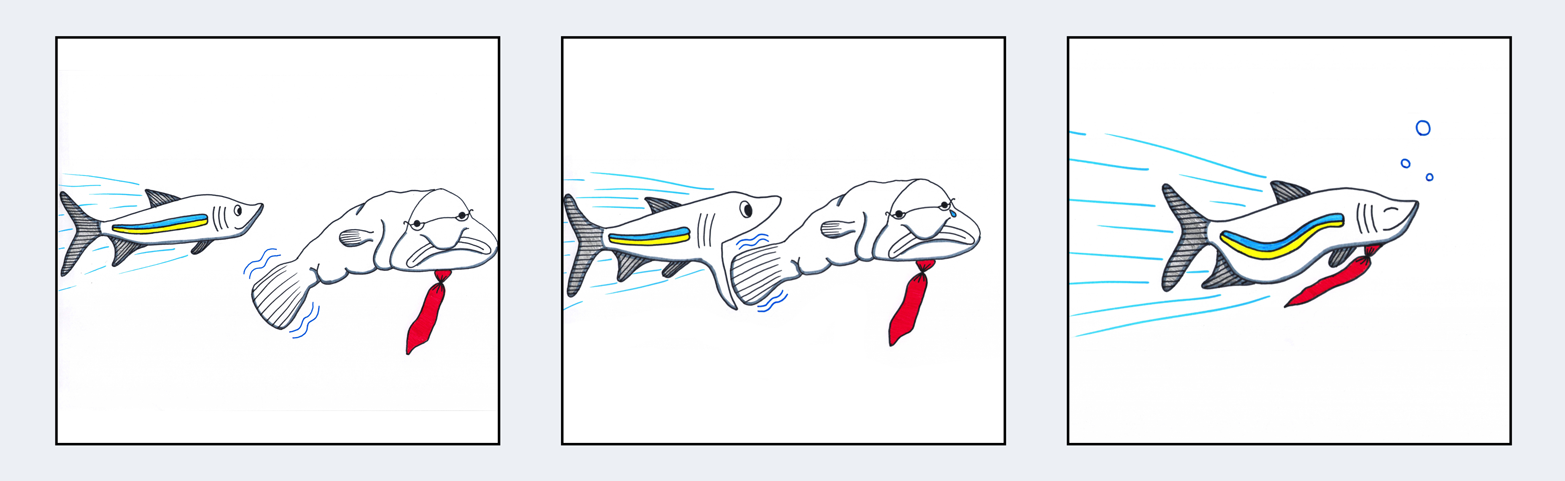
\includegraphics[width=\textwidth]{images/fast_fish.png}
	\caption{Slow fish versus fast fish \cite{rma}}
\end{figure}

One of the key benefits, for which more and more companies are adopting microservices, is the short time span between a request for change and its deployment that they offer. This is thanks to proficiency in continuous delivery.

\begin{definition}[Continuous delivery]
Continuous Delivery is a software development discipline where you build software in such a way that the software can be released to production at any time. \footnote{Continuous Delivery by Martin Fowler \url{https://martinfowler.com/bliki/ContinuousDelivery.html}}
\end{definition}

So continuous delivery enabled by continuous integration is the ability to quickly roll-out software updates to production. The biggest risk to any software effort is that you end up building something that isn't useful. Continuous delivery helps to avoid this by enabling early user feedback. Also since it`s recommended to continuously roll-out small updates to the production, there is less to go wrong and it`s easier to fix should a problem appear.

The isolation and autonomy principles empower fast and flexible microservice deployment and upgrade. They make it possible for new versions of microservices to be taken into production independently of changes to others, allowing us to safely roll-out or revert changes incrementally - service by service. What`s more we can roll the changes out instance by instance of the same microservice and slowly redirect the traffic to the new version, which effectively means zero downtime. That is a big deal for systems that have very strict availability requirements.

With the flexibility of routing and deployment it is also easy to exercise canary release. Canary release is a technique for reduction of risk, in which you expose new versions only to a fraction of the users at first. You can choose a random sample of users or you can target certain groups of people according to region, age, sex, etc. and get their feedback. And only if those users are happy with the new version, you make the update available to all users.

\subsection{Technology diversity}

Since the only relation between individual microservices should be a network communication through an agreed interface that should be language-agnostic, developers can take advantage of technology diversity. This benefit also eliminates long-term commitment to a single technology stack.

It is possible for every microservice to be written in different programming language, use different framework or even be developed for different platform like x64 or ARM. ARM architecture is usually less power consuming, which can be useful in IoT\footnote{Internet of Things - \url{https://en.wikipedia.org/wiki/Internet_of_things}} applications. Each microservice can leverage the use use of database type that is the most suitable for its data, be it relational or non-relational database.

\paragraph{The Drawbacks of Microservices}

\subsection{Architecture complexity}

While microservices take away the complexity of big monoliths they bring another type of complexity that is inherent in the microservice architecture itself. It arises from the fact microservices are distributed system, so there are many things that need to be taken care of.

The deployment environment is much more complicated. Now there is no application server, to which you simply deploy your WAR file. You need a mature operations team and employ new middleware and tools to manage numerous microservice instances, which are being redeployed regularly.

\subsection{Network communication}

Microservices heavily depend on network communication which always brings many problems to the table. There is no simple invocation of method in different module via language specific call, you have to use remote call to communicate with another microservice.

If all things work perfectly, the network call may take a multitudes of time. Even inter-process network calls between instances on the same machine take substantial amount of time compared to method call inside a single process. So developers need to find a compromise between excessive division of business functionality into individual microservices and its aggregation.

What`s more in network space you never know what can go wrong on the other side or if your message ever reach its destination, so you need to take care of every possibility. This alone brings a massive amount of complexity to microservice architecture. You need to have strong resilient mechanisms in every microservice, implement timeouts and fallbacks, and check incoming data.

\subsection{Data consistency}

Since microservice architecture promotes ownership of data associated to each microservice and not having a single database for everything, data consistency becomes a challenge.

Business transactions that update multiple business entities are fairly common. In microservice architecture these business entities can belong to different microservices. Using distributed transactions should be put to use only for critical data because of the CAP theorem\footnote{\url{https://en.wikipedia.org/wiki/CAP_theorem}}. All other data should do with eventual consistency\footnote{\url{https://en.wikipedia.org/wiki/Eventual_consistency}}.

\subsection{Testing complexity}

If we omit unit testing which verifies the workings of internal components and should have the same complexity in both cases, then microservice architecture has more complicated overall testing.

In monolithic application with modern frameworks its trivial to write tests which start the application and test its external APIs. However, with microservices you need to also test inter-service communication and application as a whole. To do that you have to launch the tested microservice and any other microservices it depends on, or their stub. You may also need to test compatibility of various versions of microservices.

\paragraph{Summary\newline\newline}

Microservice architecture is ideal for big, demanding, robust systems. The common problems that companies were facing were related to size of the system. Microservice architecture is designed to solve problems of systems which grew in size beyond the boundaries that were initially defined when the system was designed. Microservices are also ideal for applications with very high load and availability demands.

There are no silver bullets, like every other technology, microservice architecture has its advantages and disadvantages and so it`s advisable in some situations and inappropriate in others. In picture \ref{productivity} we can see fitness of microservices with regard to applications complexity.

\begin{figure}[ht!]
	\label{productivity}
	\centering
	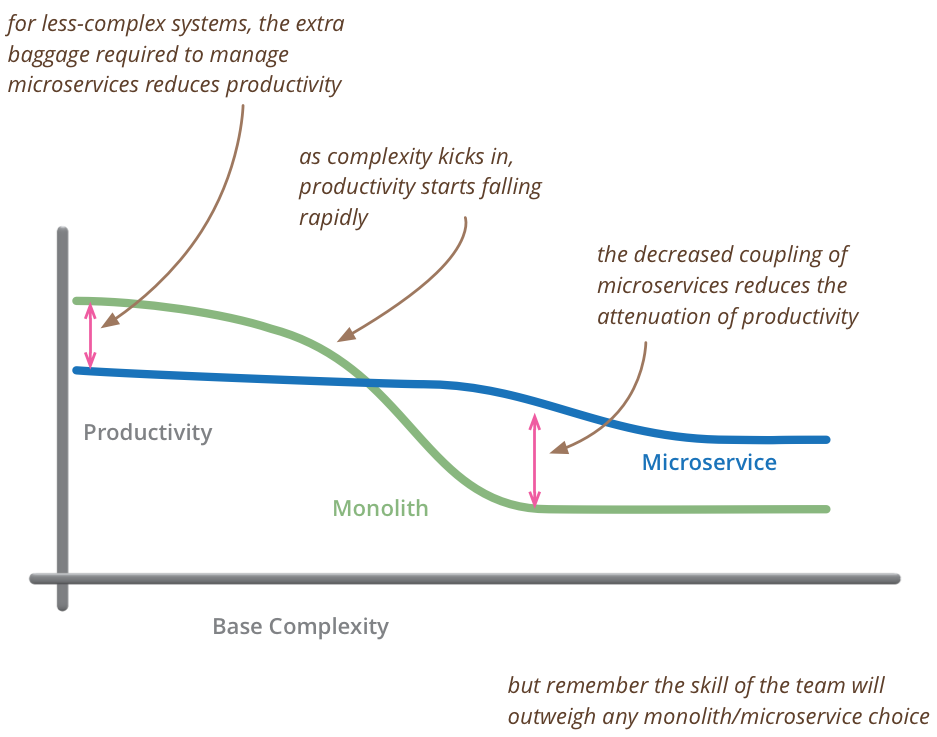
\includegraphics[width=\textwidth]{images/complexity_productivity.png}
	\caption{Relationship between complexity and productivity\footnotemark}
\end{figure}

\footnotetext{Source: \url{https://martinfowler.com/microservices/}}

\section{Containers}

In traditional approach we built one binary of our application and deployed it to the server which needed to be correctly configured (correct permissions, environment variables, etc.) and include everything that our application need for functioning. Likewise we needed to be careful so that various changes don`t impact other applications also running on the same server. With microservices this becomes much more complicated.

After we break our application we end up with many moving pieces. Services, binaries, different configurations etc. We need a technique to elegantly wrap our application to integrated packages that are easy to deploy and simultaneously segregate our application from the rest.

In the past, virtualization was used for this need. Virtual machines have their foundation in some areas, but they are cumbersome. Each virtual machine virtualizes an entire hardware. Images of virtual machines are huge because they not only contain the application but the whole operating system with the required drivers and other redundant parts. Virtual machines are hard to manage, patch, and change.

With the takeoff of microservices we were in need of better solution, which would pose less overhead.

The reason microservice architecture is financially and operationally feasible has a lot to do with containers.

Once you have packaged your service as a container image, you then launch one or more containers. You usually run multiple containers on each physical or virtual host.

You might use a cluster manager such as Kubernetes or Marathon to manage your containers.

\section{Existing frameworks and solutions}

\section{SilverWare}

\chapter{Monitoring of microservices}

\bibliographystyle{IEEEtran}
\bibliography{sources}
\end{document}
